\chapter{Procedures and Implementation Methods}

This chapter presents the operating procedures of the CyberCase Intelligence Framework, from case intake and source storage to case analysis, follow-up questions, analysis display, and preliminary report generation. It describes the system from the user's perspective together with the process, architecture, and database designs that support the implementation. The design keeps analytical inputs traceable to their original sources and clearly separates external knowledge from case facts.

\section{System Overview}

The user registers or signs in, then creates a case and assigns a title to establish a dedicated workspace.

The user can add case sources in two forms: a directly typed case narrative or an uploaded document or image.

The system validates file type and size. Text-based PDFs are read from their text layer, PDFs without usable text are rendered as images for document recognition, and DOCX files are read from paragraphs and tables.

Imported text is stored as a document and a case source together with provenance such as the filename, extraction method, page number, and ingestion warnings.

When the user requests analysis, the system reads the case source bundle and follow-up history, then assesses missing information before deciding whether to ask a question or continue analysis.

When an important askable gap is found, the system creates a focused follow-up question and displays it in the chat area. The answer is stored as a conversation message that can be read by the next analysis, but it is not automatically promoted to a case source.

When no follow-up is required, the system assesses whether the case has relevant MITRE ATT\&CK context. The RAG service is called only when the case passes the technical relevance gate; otherwise, that stage is skipped.

The system sends admitted sources and permitted context to the language model to create a structured analysis, then validates source identifiers and quoted text against the sources that actually belong to the case.

A validated analysis is stored as the current analysis result for the case. The user can view the summary, findings, timeline, gaps, and source references.

A preliminary report is generated from the stored analysis and can be displayed as HTML or exported as PDF. MITRE information is presented as technical context separated from the case facts.

\begin{figure}[H]
\centering
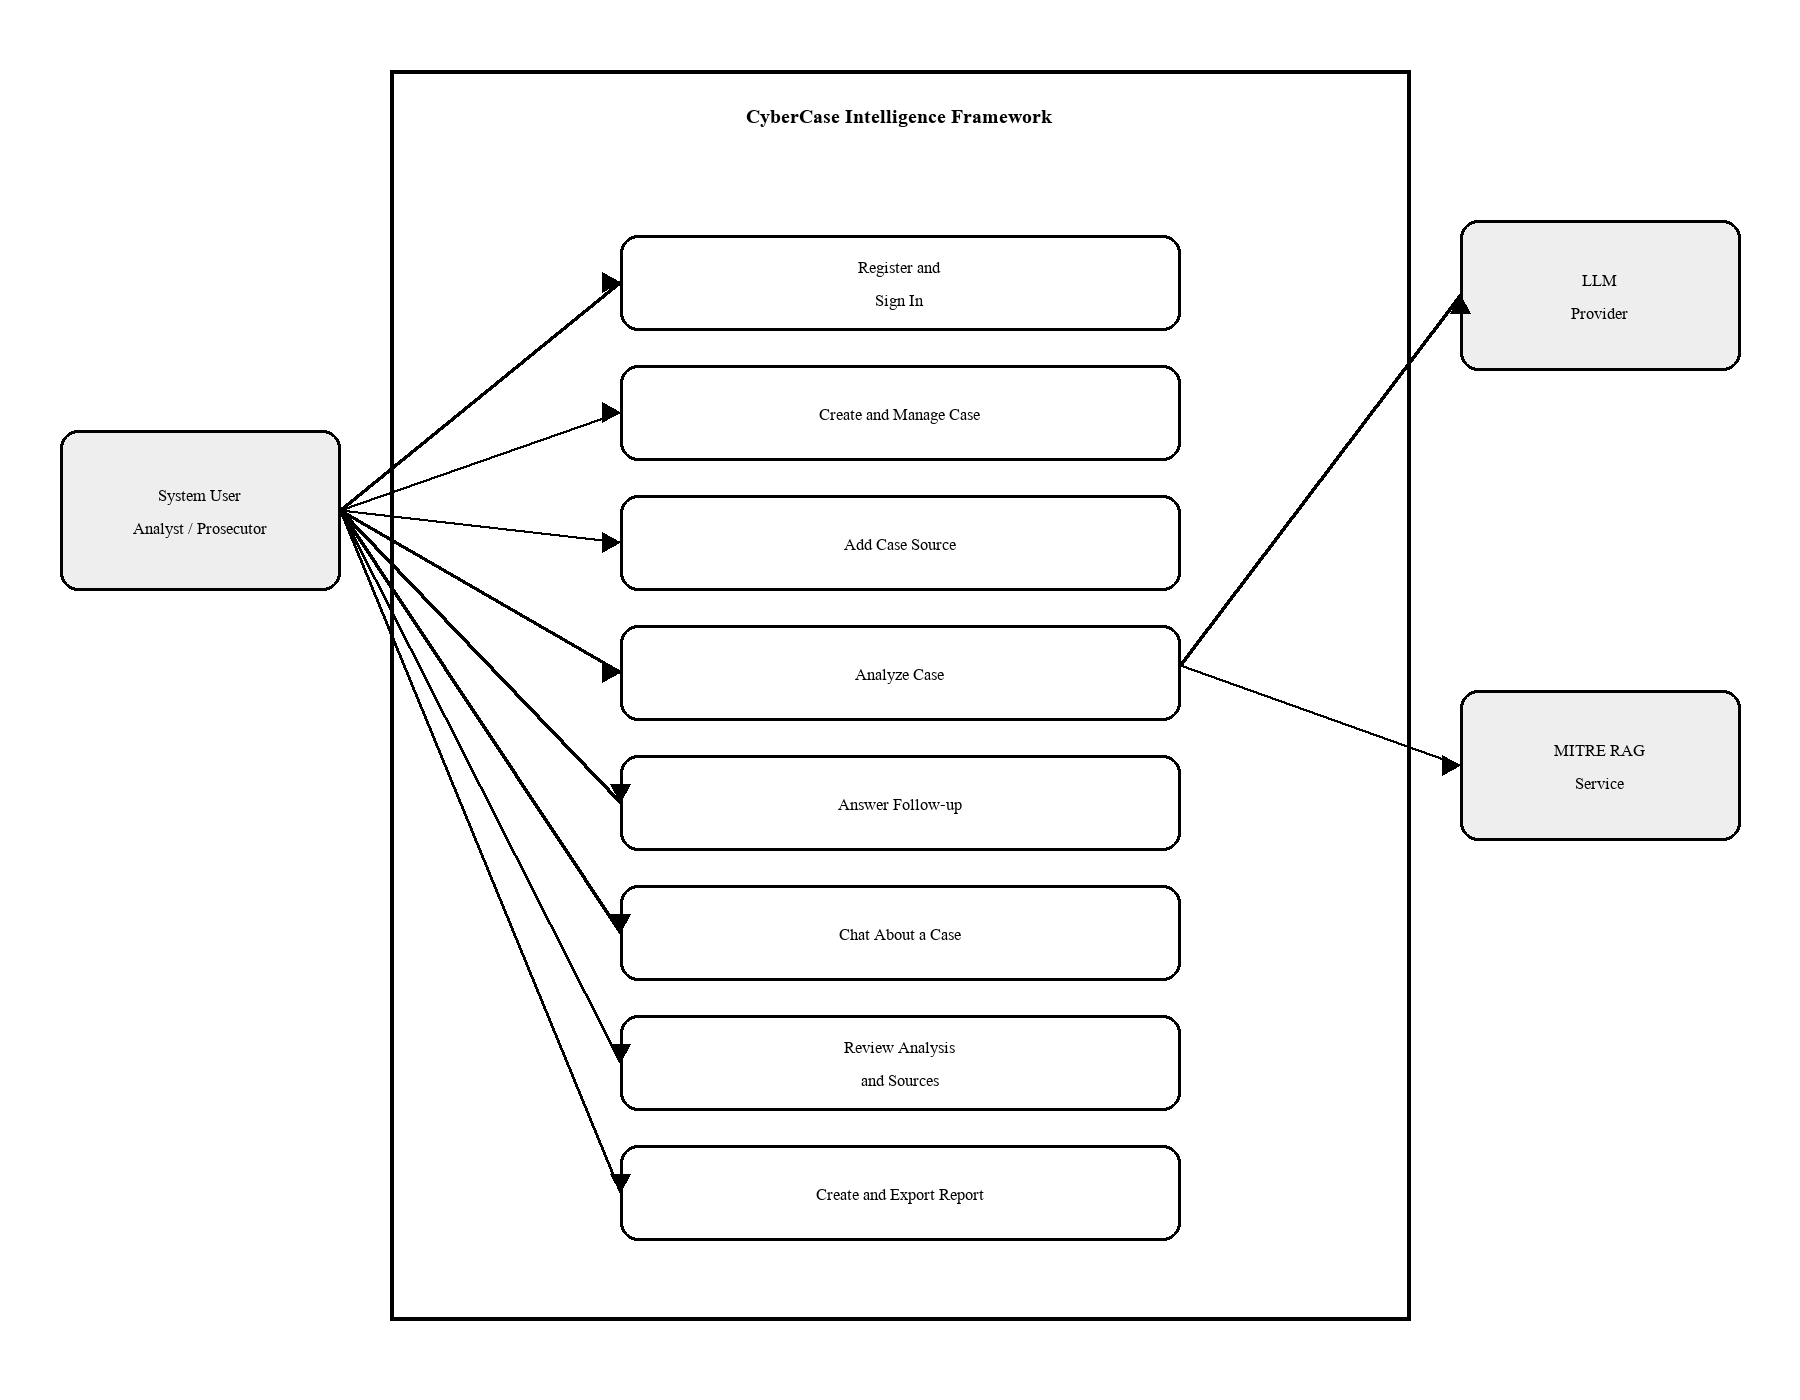
\includegraphics[width=0.96\textwidth]{figures/chapter3/figure-3-1.png}
\caption{Use Case Diagram of the CyberCase Intelligence Framework}\label{fig:3-1}
\end{figure}

\section{Use Case Description}

\begin{longtable}{@{}>{\raggedright\arraybackslash}p{0.20\textwidth} >{\raggedright\arraybackslash}p{0.30\textwidth} >{\raggedright\arraybackslash}p{0.46\textwidth}@{}}
\caption{Use Case Description Register and Sign In}\label{tab:3-1}\\
\toprule
\textbf{Use Case Name} & \textbf{Register and Sign In} & \textbf{} \\
\midrule
\endfirsthead
\textbf{Use Case Name} & \textbf{Register and Sign In} & \textbf{} \\
\midrule
\endhead
Actor & System User &  \\
Purpose & Authenticate the user before providing access to the workspace and the user's cases. &  \\
Related Use Cases & - Create and Manage Case \newline - Add Case Source &  \\
Pre-Conditions & - User account data exists or registration data is provided \newline - The system can connect to the database &  \\
Post-Conditions & - The user can enter the workspace \newline - Case access is restricted to the user's account &  \\
Flow of Event & User \newline 1. Enter account information \newline 2. Select Register or Sign In & System \newline 1. Validate account format and data \newline 2. Store the account or create a session \newline 3. Navigate to the case list \\
Exception & Missing data, a duplicate account, or invalid credentials prevent the operation from continuing. &  \\
\bottomrule
\end{longtable}

\begin{longtable}{@{}>{\raggedright\arraybackslash}p{0.20\textwidth} >{\raggedright\arraybackslash}p{0.30\textwidth} >{\raggedright\arraybackslash}p{0.46\textwidth}@{}}
\caption{Use Case Description Create and Manage Case}\label{tab:3-2}\\
\toprule
\textbf{Use Case Name} & \textbf{Create and Manage Case} & \textbf{} \\
\midrule
\endfirsthead
\textbf{Use Case Name} & \textbf{Create and Manage Case} & \textbf{} \\
\midrule
\endhead
Actor & System User &  \\
Purpose & Create a workspace for collecting sources and analysis results for one case. &  \\
Related Use Cases & - Register and Sign In \newline - Add Case Source \newline - Analyze Case &  \\
Pre-Conditions & - The user is signed in \newline - The case title satisfies the system constraints &  \\
Post-Conditions & - The user can view, rename, or delete cases according to the user's permissions &  \\
Flow of Event & User \newline 1. Select a new case or an existing case \newline 2. Enter or edit the case title \newline 3. Open the selected case & System \newline 1. Create or update the case record \newline 2. Show the analysis freshness status when sources change \\
Exception & If the case is not found or the user lacks access, the system cancels the operation and reports an error. &  \\
\bottomrule
\end{longtable}

\begin{longtable}{@{}>{\raggedright\arraybackslash}p{0.20\textwidth} >{\raggedright\arraybackslash}p{0.30\textwidth} >{\raggedright\arraybackslash}p{0.46\textwidth}@{}}
\caption{Use Case Description Add Case Source}\label{tab:3-3}\\
\toprule
\textbf{Use Case Name} & \textbf{Add Case Source} & \textbf{} \\
\midrule
\endfirsthead
\textbf{Use Case Name} & \textbf{Add Case Source} & \textbf{} \\
\midrule
\endhead
Actor & System User &  \\
Purpose & Add text or a document that the system can use as an input source for case analysis. &  \\
Related Use Cases & - Create and Manage Case \newline - Review Sources \newline - Analyze Case &  \\
Pre-Conditions & - The user owns the case \newline - The text is non-empty or the file type is supported &  \\
Post-Conditions & - The source is stored with provenance \newline - The case source revision is updated &  \\
Flow of Event & User \newline 1. Type a case narrative or select a PDF, DOCX, PNG, or JPEG file \newline 2. Confirm the source submission & System \newline 1. Validate the type and size \newline 2. Read the text or call document recognition when necessary \newline 3. Store the document, extraction result, and case source \\
Exception & An empty, oversized, unreadable, or unsupported file does not create an incomplete case source. &  \\
\bottomrule
\end{longtable}

\begin{longtable}{@{}>{\raggedright\arraybackslash}p{0.20\textwidth} >{\raggedright\arraybackslash}p{0.30\textwidth} >{\raggedright\arraybackslash}p{0.46\textwidth}@{}}
\caption{Use Case Description Analyze Case}\label{tab:3-4}\\
\toprule
\textbf{Use Case Name} & \textbf{Analyze Case} & \textbf{} \\
\midrule
\endfirsthead
\textbf{Use Case Name} & \textbf{Analyze Case} & \textbf{} \\
\midrule
\endhead
Actor & System User, LLM Provider, MITRE RAG Service &  \\
Purpose & Create a preliminary summary and analysis from case sources with references back to the source text. &  \\
Related Use Cases & - Add Case Source \newline - Answer Follow-up Question \newline - Review Analysis \newline - Create and Export Report &  \\
Pre-Conditions & - Readable case sources are available \newline - The user selects an output language \newline - Required providers are reachable &  \\
Post-Conditions & - The system returns either a follow-up-required state or a validated analysis \newline - The analysis is bound to the source revision used to create it &  \\
Flow of Event & User \newline 1. Select Analyze Case \newline 2. Wait for the result or open the follow-up question created by the system & System \newline 1. Read case sources and follow-up history \newline 2. Assess gaps and apply the decision policy \newline 3. Call MITRE RAG only after the relevance gate \newline 4. Create a structured analysis \newline 5. Validate source IDs and quoted text \newline 6. Store the result \\
Exception & If the assessment or model does not return the required contract, the system reports the cause and does not store an unvalidated result. &  \\
\bottomrule
\end{longtable}

\begin{longtable}{@{}>{\raggedright\arraybackslash}p{0.20\textwidth} >{\raggedright\arraybackslash}p{0.30\textwidth} >{\raggedright\arraybackslash}p{0.46\textwidth}@{}}
\caption{Use Case Description Answer Follow-up Question}\label{tab:3-5}\\
\toprule
\textbf{Use Case Name} & \textbf{Answer Follow-up Question} & \textbf{} \\
\midrule
\endfirsthead
\textbf{Use Case Name} & \textbf{Answer Follow-up Question} & \textbf{} \\
\midrule
\endhead
Actor & System User &  \\
Purpose & Fill an important information gap before the system continues case analysis. &  \\
Related Use Cases & - Analyze Case \newline - Review Analysis &  \\
Pre-Conditions & - An unanswered follow-up question exists \newline - The user is working in the case associated with the question &  \\
Post-Conditions & - The answer is stored as a conversation message linked to the question \newline - The system shows the next question or starts the next analysis round when the round is complete &  \\
Flow of Event & User \newline 1. Read the follow-up question \newline 2. Enter the answer \newline 3. Submit the answer & System \newline 1. Check the outstanding question \newline 2. Store the answer and its relationship to the question \newline 3. Select the next question or start the next analysis round within the budget \\
Exception & If the question has already been answered or the request is duplicated, the system returns the existing response and does not create a duplicate message. &  \\
\bottomrule
\end{longtable}

\begin{longtable}{@{}>{\raggedright\arraybackslash}p{0.20\textwidth} >{\raggedright\arraybackslash}p{0.30\textwidth} >{\raggedright\arraybackslash}p{0.46\textwidth}@{}}
\caption{Use Case Description Chat About a Case}\label{tab:3-6}\\
\toprule
\textbf{Use Case Name} & \textbf{Chat About a Case} & \textbf{} \\
\midrule
\endfirsthead
\textbf{Use Case Name} & \textbf{Chat About a Case} & \textbf{} \\
\midrule
\endhead
Actor & System User, LLM Provider &  \\
Purpose & Allow the user to ask general questions about a case using the available analysis or sources. &  \\
Related Use Cases & - Analyze Case \newline - Review Analysis &  \\
Pre-Conditions & - The user can access the case \newline - The question is non-empty &  \\
Post-Conditions & - User and assistant messages are stored in order \newline - Chat messages are not automatically treated as case sources &  \\
Flow of Event & User \newline 1. Type a question in the chat area \newline 2. Submit the message & System \newline 1. Build context from the latest analysis or the case sources \newline 2. Call the language model \newline 3. Store the question and answer as case messages \\
Exception & A repeated request with the same client request identifier returns the existing response to prevent duplicate data. &  \\
\bottomrule
\end{longtable}

\begin{longtable}{@{}>{\raggedright\arraybackslash}p{0.20\textwidth} >{\raggedright\arraybackslash}p{0.30\textwidth} >{\raggedright\arraybackslash}p{0.46\textwidth}@{}}
\caption{Use Case Description Review Analysis and Sources}\label{tab:3-7}\\
\toprule
\textbf{Use Case Name} & \textbf{Review Analysis and Sources} & \textbf{} \\
\midrule
\endfirsthead
\textbf{Use Case Name} & \textbf{Review Analysis and Sources} & \textbf{} \\
\midrule
\endhead
Actor & System User &  \\
Purpose & Read the analysis and inspect the source text that supports the system's findings. &  \\
Related Use Cases & - Analyze Case \newline - Add Case Source &  \\
Pre-Conditions & - A validated analysis or a source list is available \newline - The user is in the correct case &  \\
Post-Conditions & - The system displays the available summary, findings, timeline, gaps, and technical context \newline - Source text can be opened with document and page information when available &  \\
Flow of Event & User \newline 1. Open the analysis or sources page \newline 2. Select a finding or citation to inspect & System \newline 1. Read the API response \newline 2. Match source IDs to case sources \newline 3. Display quoted text and provenance \newline 4. Separate MITRE context from case facts \\
Exception & If the analysis does not match the latest source revision, the system shows a stale status and does not present the old result as current. &  \\
\bottomrule
\end{longtable}

\begin{longtable}{@{}>{\raggedright\arraybackslash}p{0.20\textwidth} >{\raggedright\arraybackslash}p{0.30\textwidth} >{\raggedright\arraybackslash}p{0.46\textwidth}@{}}
\caption{Use Case Description Create and Export Report}\label{tab:3-8}\\
\toprule
\textbf{Use Case Name} & \textbf{Create and Export Report} & \textbf{} \\
\midrule
\endfirsthead
\textbf{Use Case Name} & \textbf{Create and Export Report} & \textbf{} \\
\midrule
\endhead
Actor & System User &  \\
Purpose & Create a preliminary report from a stored analysis and export it in a usable format. &  \\
Related Use Cases & - Review Analysis and Sources &  \\
Pre-Conditions & - A validated analysis exists \newline - The analysis remains bound to the correct case and source revision &  \\
Post-Conditions & - A versioned report is linked to the analysis \newline - The user can view HTML or download a PDF &  \\
Flow of Event & User \newline 1. Select Create Report \newline 2. Preview the report or export it as PDF & System \newline 1. Assemble report sections from the analysis \newline 2. Validate the structure and source IDs \newline 3. Store the report and render the selected format \\
Exception & If no current analysis exists or the report structure fails validation, the system does not create an incomplete report. &  \\
\bottomrule
\end{longtable}

\section{Flowchart}

\subsection{Registration and Sign In}

At the start of a session, the user must register or sign in. The system validates the submitted data and creates a session when the data is valid. After sign-in, the user sees only cases that the account is authorized to access. Missing data, duplicate accounts, or invalid credentials stop the operation and produce an error for correction.

\begin{figure}[H]
\centering
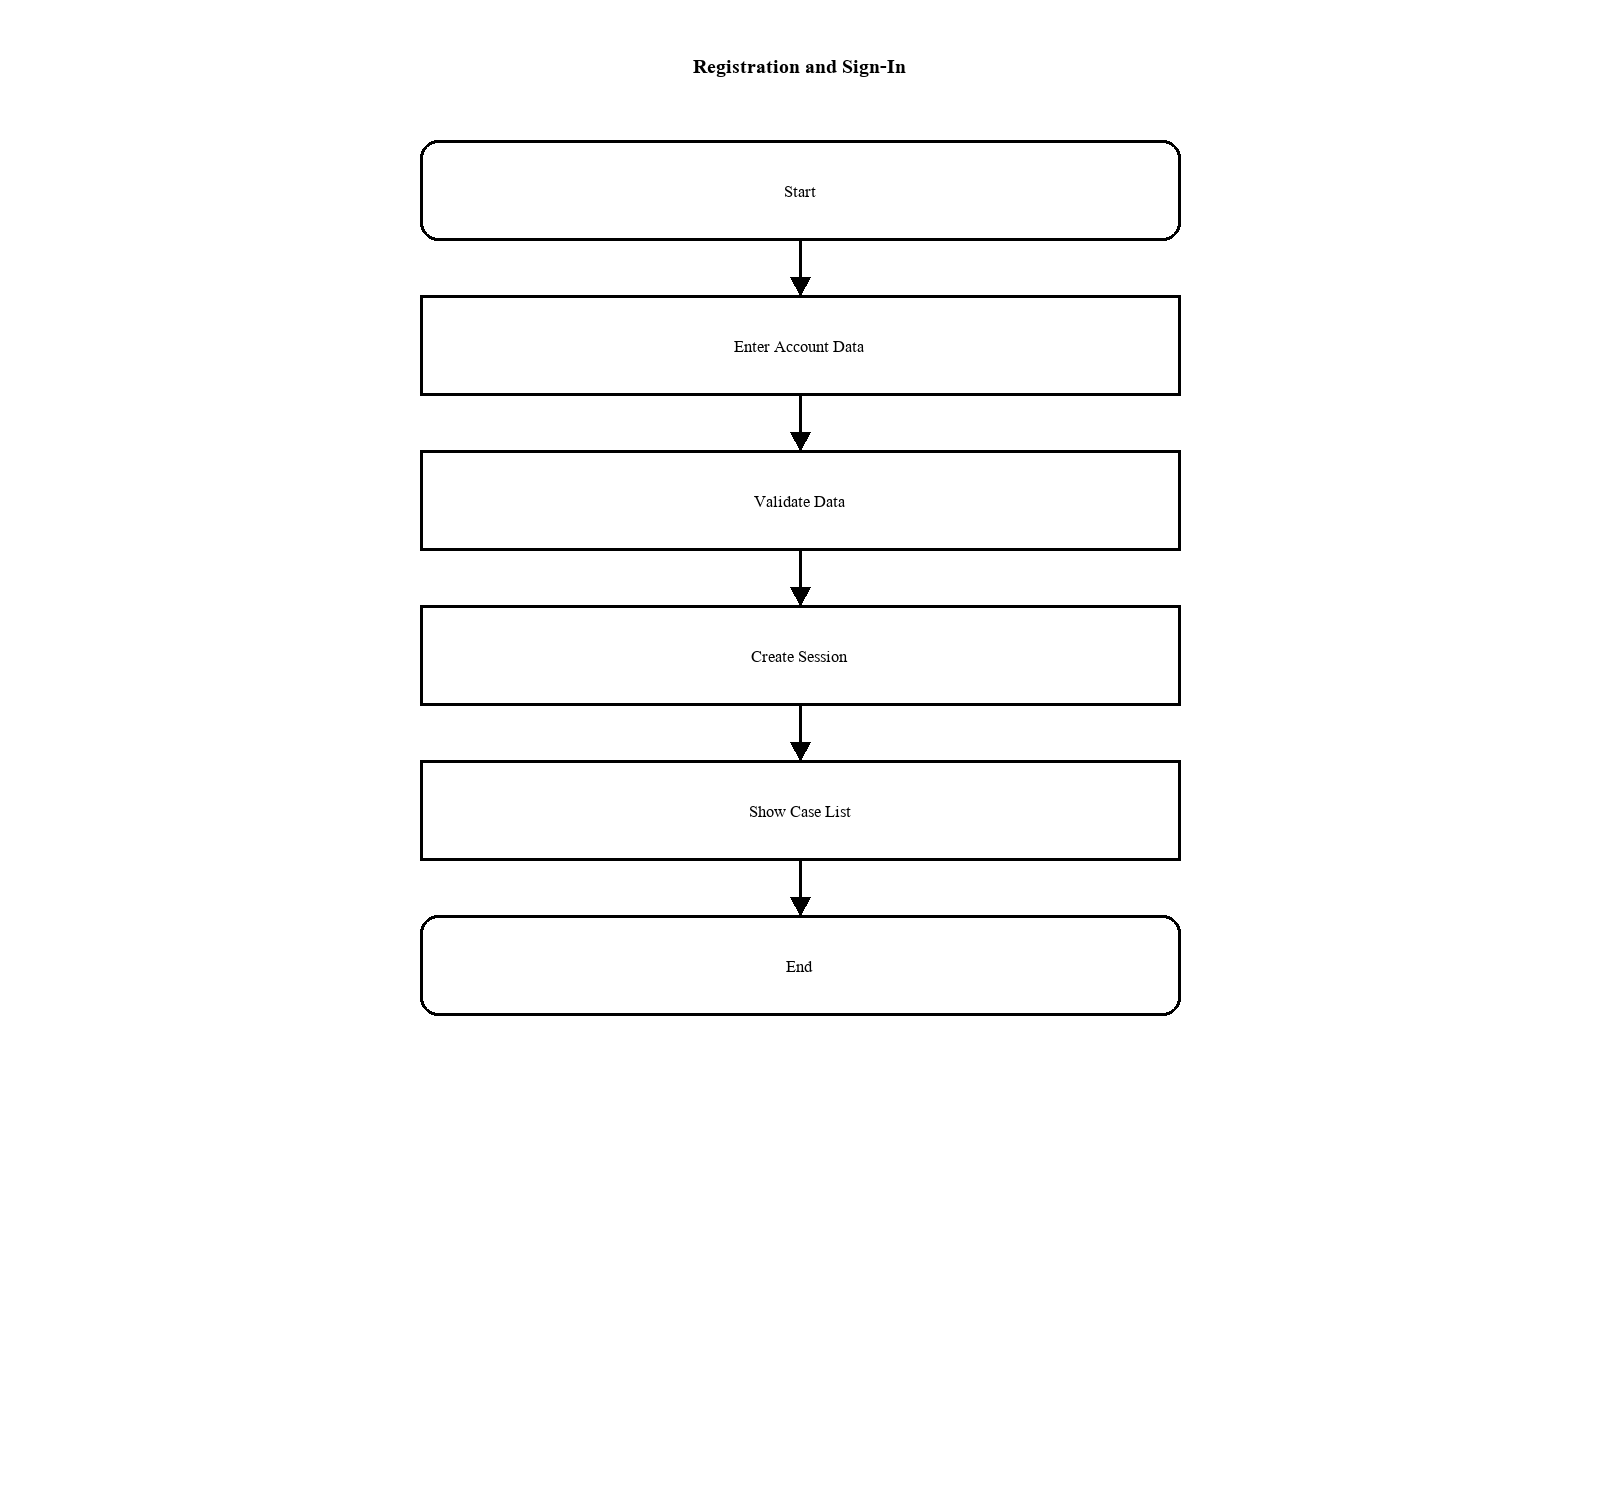
\includegraphics[width=0.96\textwidth]{figures/chapter3/figure-3-2.png}
\caption{Registration and Sign-In Flowchart}\label{fig:3-2}
\end{figure}

\subsection{Case Creation and Source Intake}

The user creates a case and adds either narrative text or a document. The system validates the file before reading it. A text-based PDF uses its existing text layer, while a PDF with insufficient text is rendered as an image for page-level document recognition. DOCX files are read from paragraphs and tables, and images are sent to document recognition. The system then stores the extracted text with the extraction method, page number, warnings, and relationship to the original document.

\begin{figure}[H]
\centering
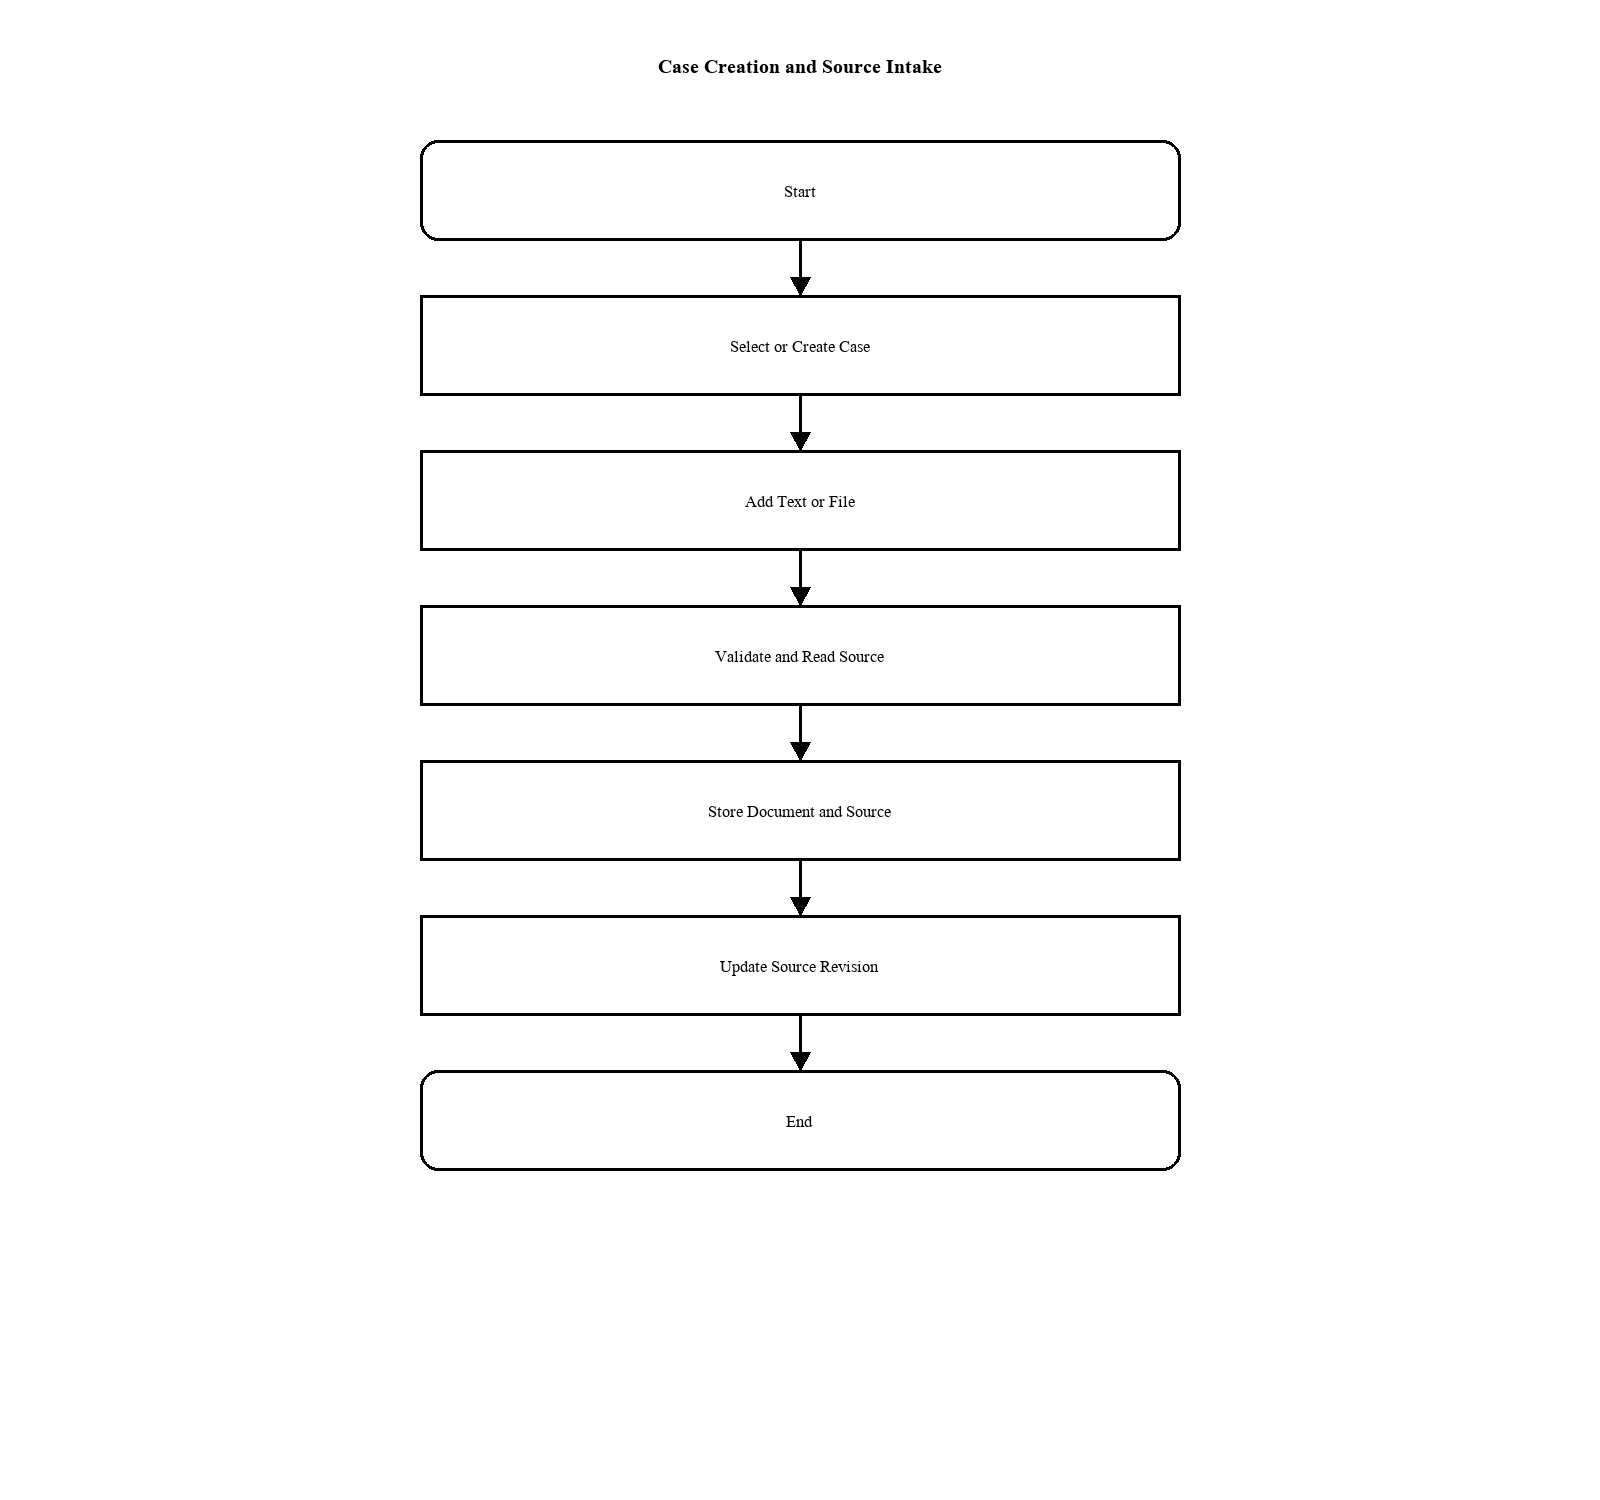
\includegraphics[width=0.96\textwidth]{figures/chapter3/figure-3-3.png}
\caption{Case-Creation and Source-Intake Flowchart}\label{fig:3-3}
\end{figure}

\subsection{Case Analysis and Follow-up}

Analysis starts by reading the case source bundle and follow-up history. The system runs the gap assessment first. If an important askable gap exists, it creates a follow-up question and waits for the answer. When the questions in the round are complete, or when no gap should be asked, the system evaluates MITRE ATT\&CK relevance and retrieves external context only when the gate allows it. The language model then creates the analysis, after which the system validates every source ID and exact quote against the sources that actually exist in the case.

\begin{figure}[H]
\centering
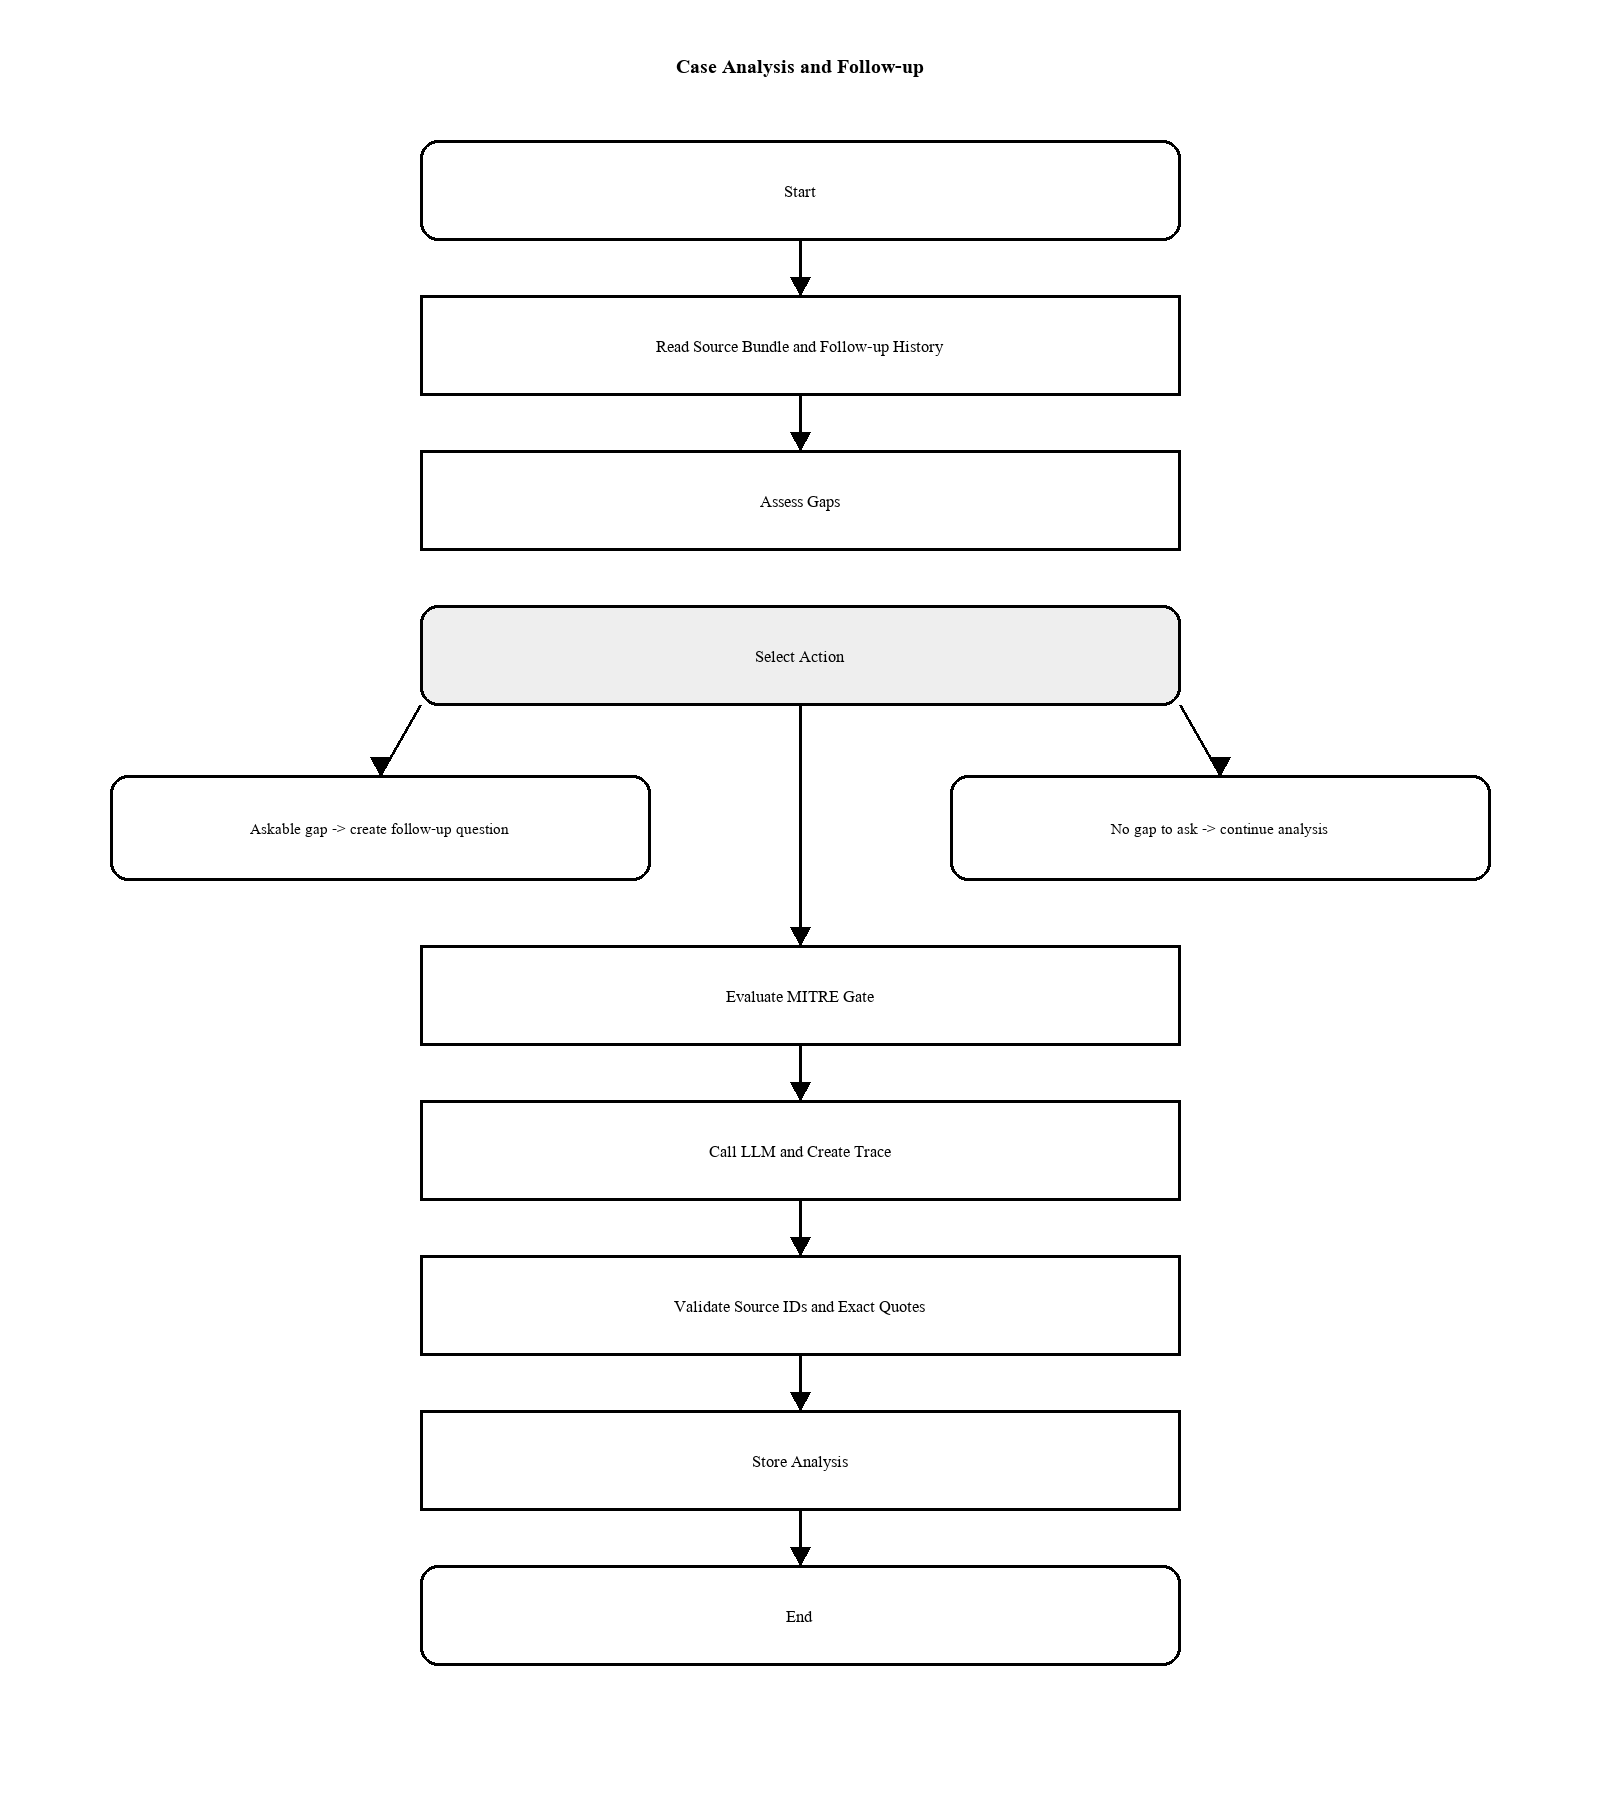
\includegraphics[width=0.96\textwidth]{figures/chapter3/figure-3-4.png}
\caption{Case-Analysis and Follow-up Flowchart}\label{fig:3-4}
\end{figure}

\subsection{Case Chat and Follow-up Answers}

The chat area supports both general questions and answers to follow-up questions. When no follow-up question is outstanding, the system builds context from the latest analysis or the case sources and sends it to the language model. When a follow-up question is outstanding, the message is stored directly as that question's answer, and the system selects the next question or starts a new analysis round according to the defined policy. Chat messages and follow-up answers therefore support analysis but are not automatically converted into case sources.

\begin{figure}[H]
\centering
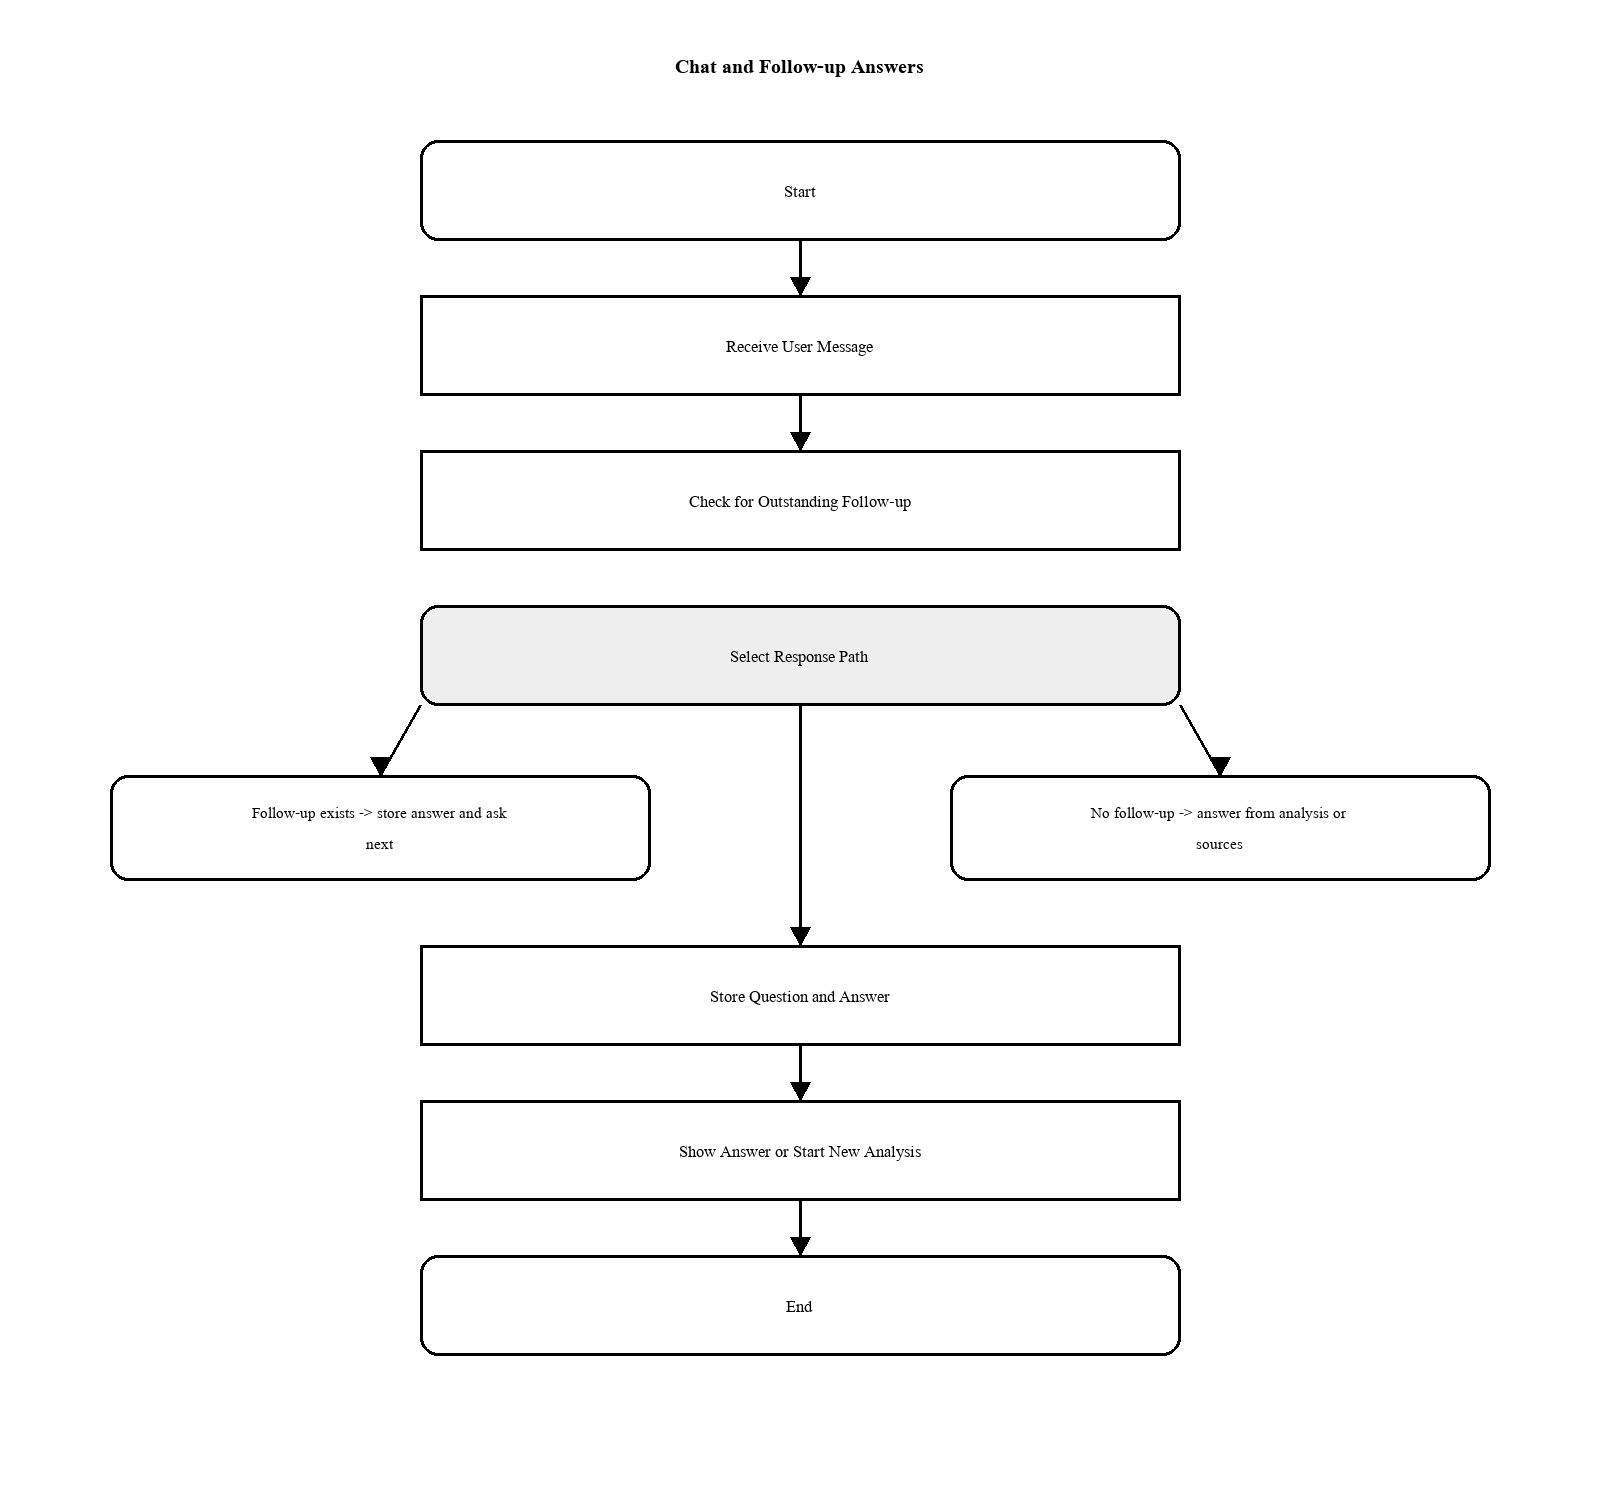
\includegraphics[width=0.96\textwidth]{figures/chapter3/figure-3-5.png}
\caption{Chat and Follow-up Answer Flowchart}\label{fig:3-5}
\end{figure}

\subsection{Report Creation and Export}

When a validated analysis is available, the user requests a report. The system assembles the preliminary report structure from stored data and does not call the language model to write the report again. The report is linked to the analysis and receives a case-level version number. The user can view it as HTML or export it as PDF, while MITRE ATT\&CK content remains technical context separated from the case facts.

\begin{figure}[H]
\centering
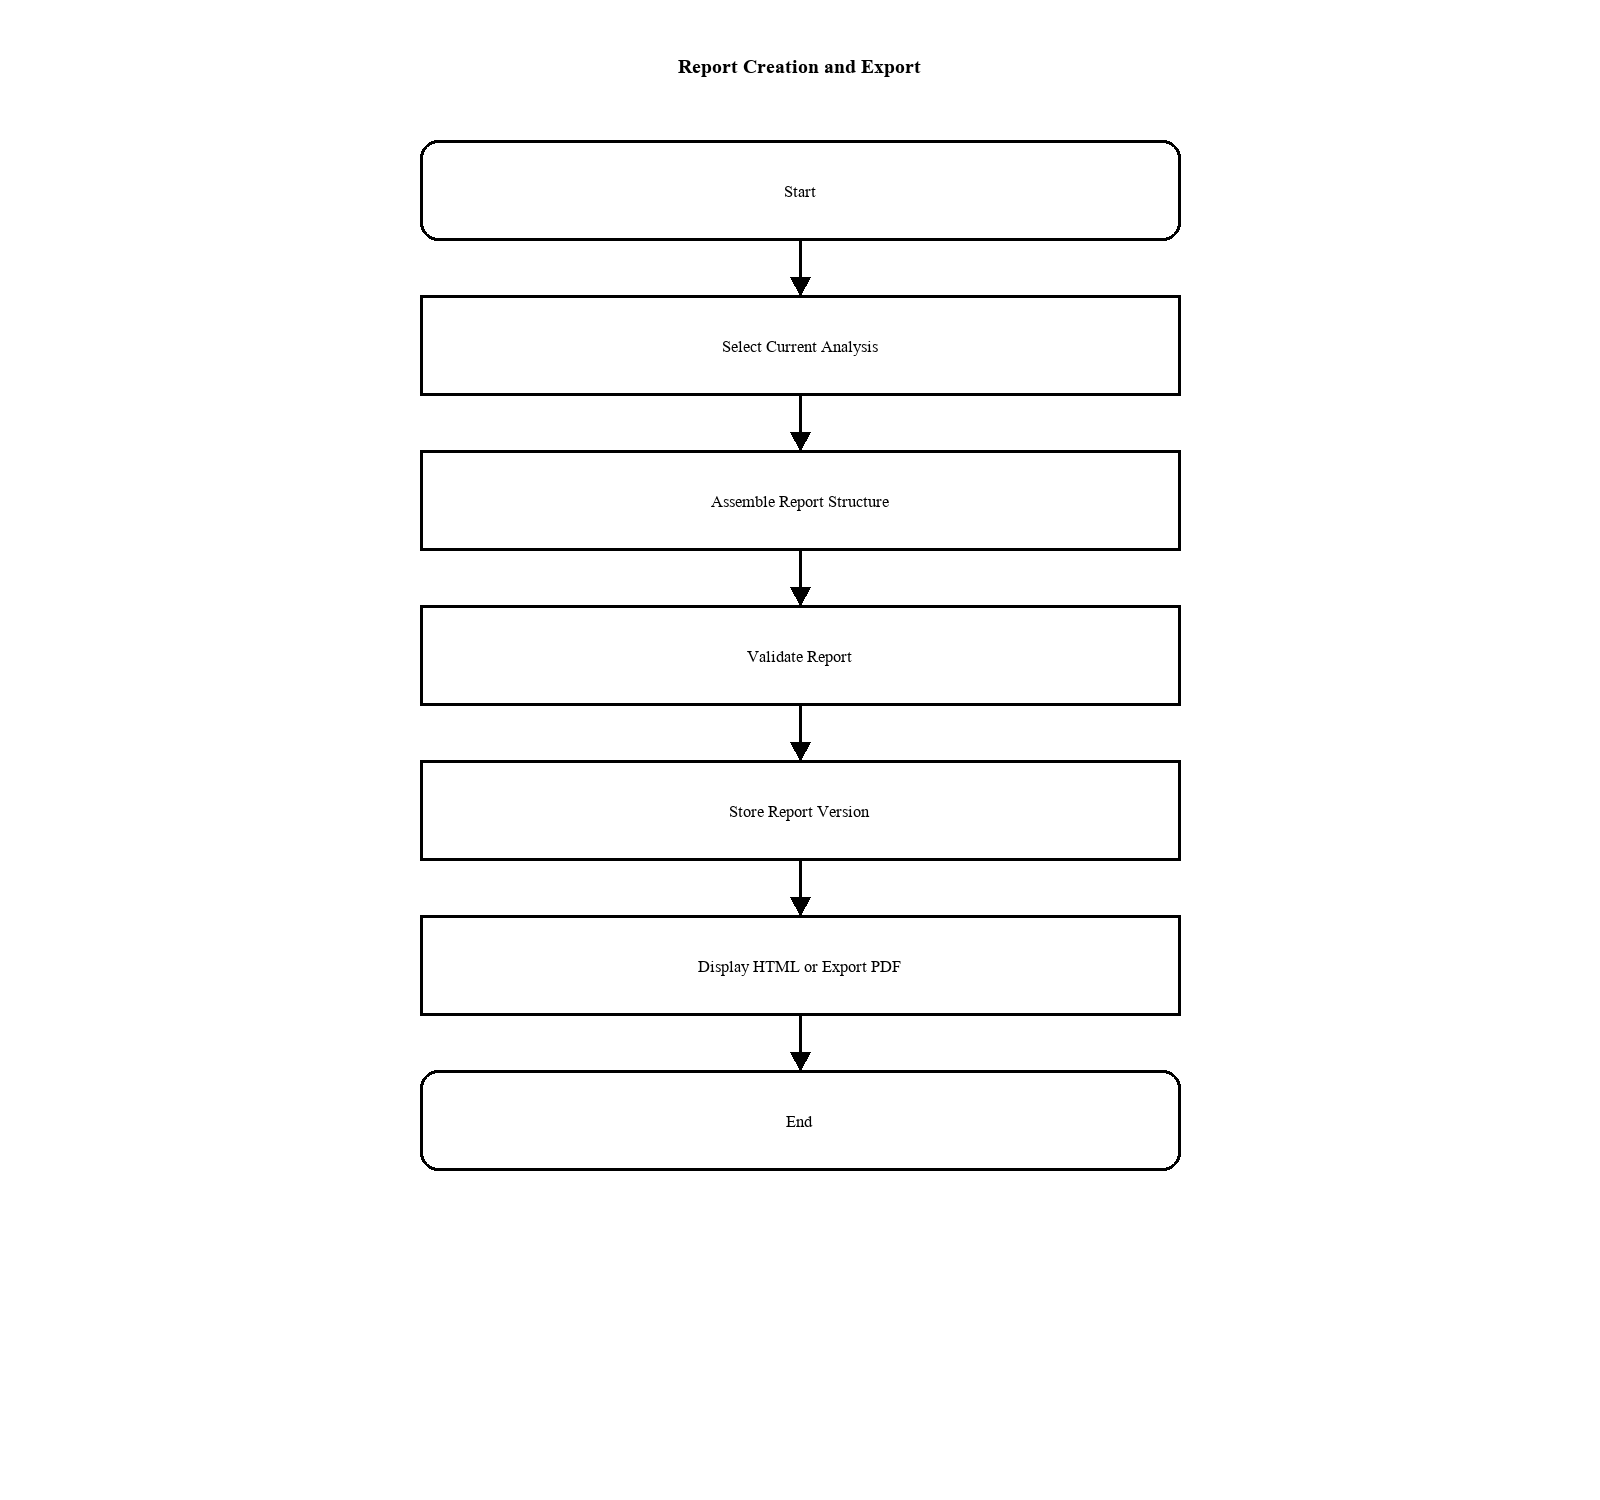
\includegraphics[width=0.96\textwidth]{figures/chapter3/figure-3-6.png}
\caption{Report-Creation and Export Flowchart}\label{fig:3-6}
\end{figure}

\section{System Architecture Design}

CyberCase is designed as a web system that separates the presentation layer, API layer, case workflow, and external services. This separation makes it easier to validate case data and distinguish the role of case sources from external knowledge.

\begin{figure}[H]
\centering
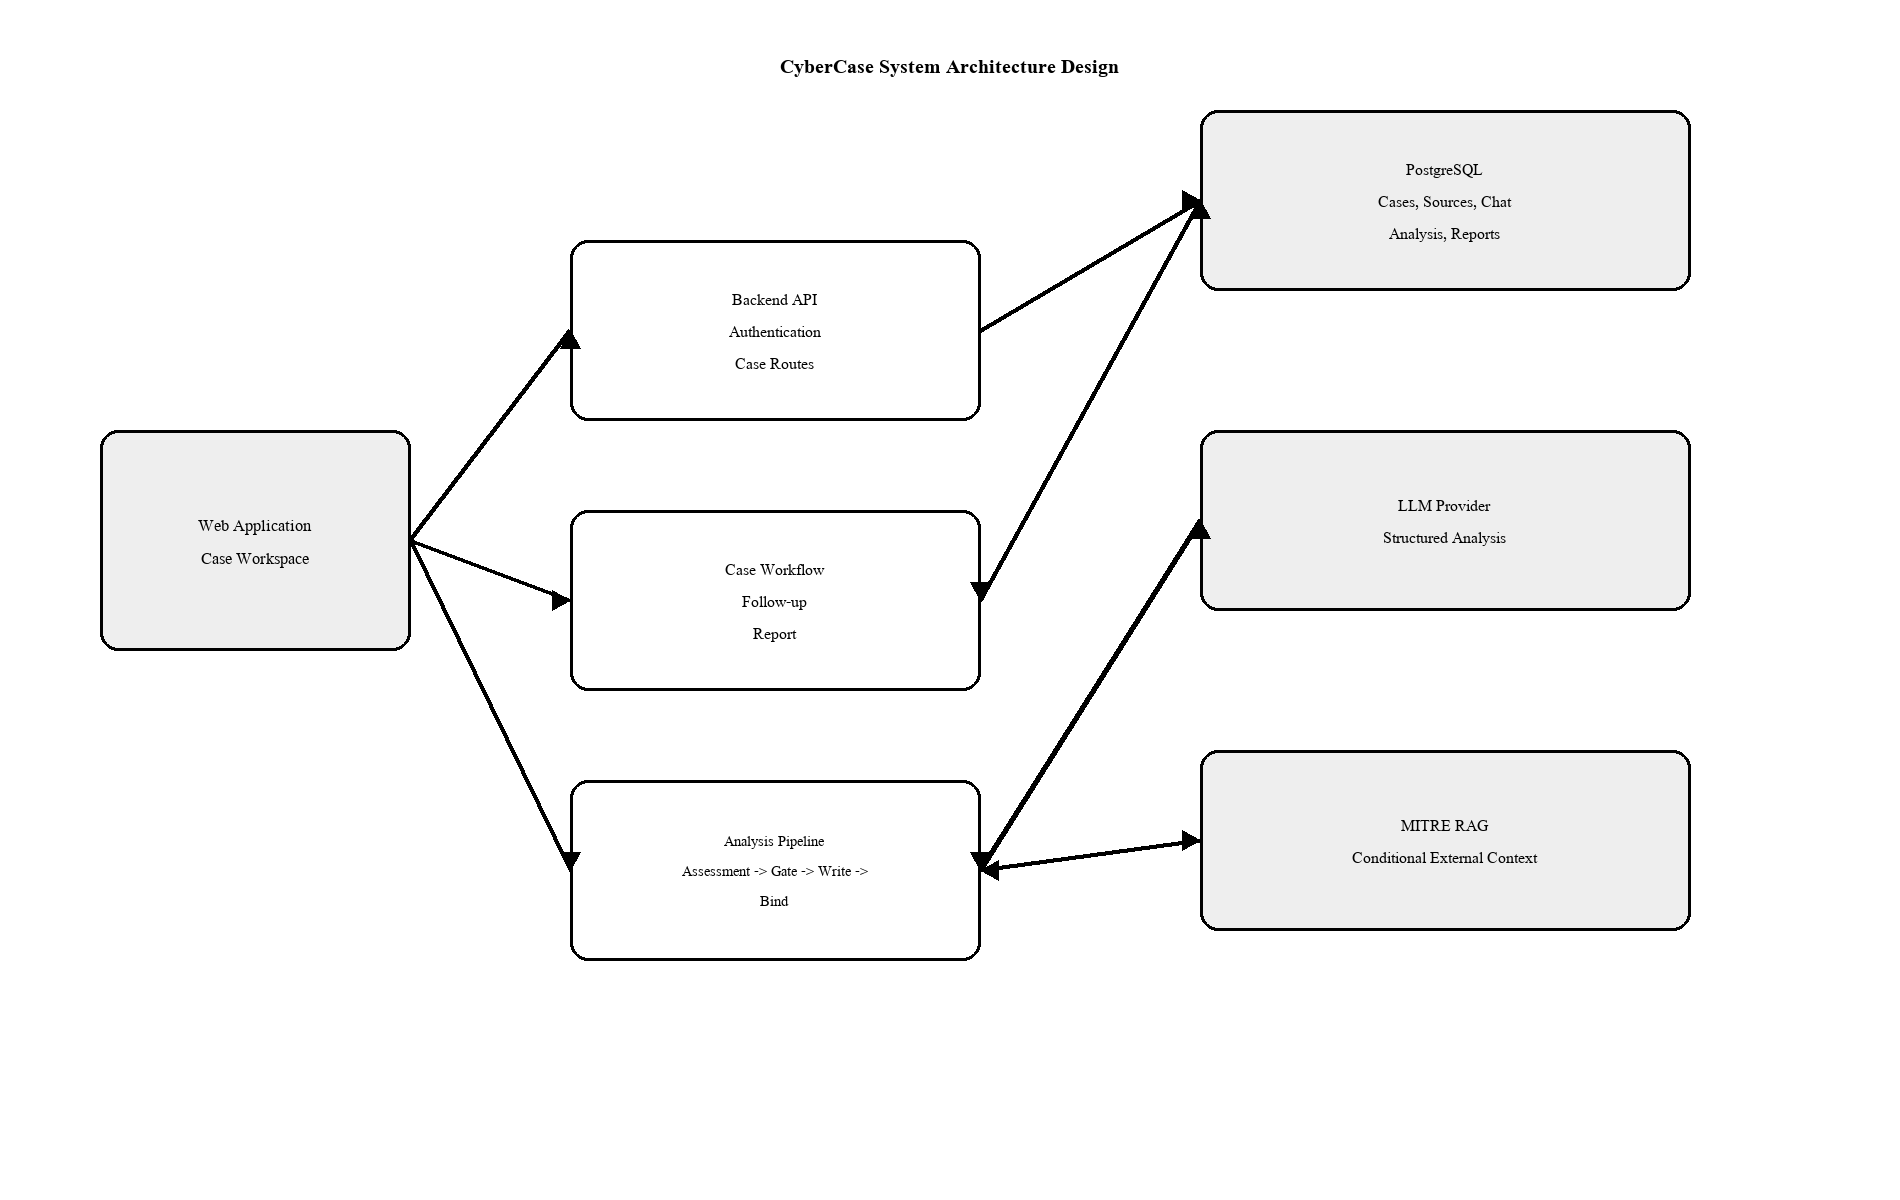
\includegraphics[width=0.96\textwidth]{figures/chapter3/figure-3-7.png}
\caption{Overview of the CyberCase System Architecture Design}\label{fig:3-7}
\end{figure}

\noindent\textbf{1)} The user works through the Web Application, which provides the case list, source management, analysis, and chat areas.

\noindent\textbf{2)} The Backend API receives requests, checks authorization, transforms data according to the API contract, and invokes the case workflow. Database reads are kept separate from the interval in which the model is processing.

\noindent\textbf{3)} The Workflow and Analysis Pipeline read the source bundle, follow-up history, and reusable context, then perform gap assessment, conditional technical augmentation, structured analysis, and citation binding back to the sources.

\noindent\textbf{4)} PostgreSQL stores user accounts, cases, documents, extraction results, case sources, chat messages, analysis results, and reports. The Case is the center of these relationships.

\noindent\textbf{5)} The LLM provider assesses gaps, creates follow-up questions, answers general questions, and creates structured analysis. The question-selection policy, round limits, and source-ID validation are deterministic Backend responsibilities.

\noindent\textbf{6)} The MITRE RAG service is an external service called only when the gate identifies relevant technical context. If it fails, the system can retain the general analysis and report the technical augmentation status separately.

\section{Database}

The system uses PostgreSQL and places the Case at the center of the data associated with one investigation. The main relationships allow one user to own multiple cases, one case to contain multiple documents and case sources, and one document to have multiple extraction results. Chat messages, analysis results, and reports are all linked back to the same case.

Case sources store the exact text used for analysis together with separate provenance data. Analysis results store the source revision used to create them, allowing the system to determine whether a result is current or stale after new sources are added. Each report is linked to the analysis that created it so that the report's origin remains explicit.

\begin{figure}[H]
\centering
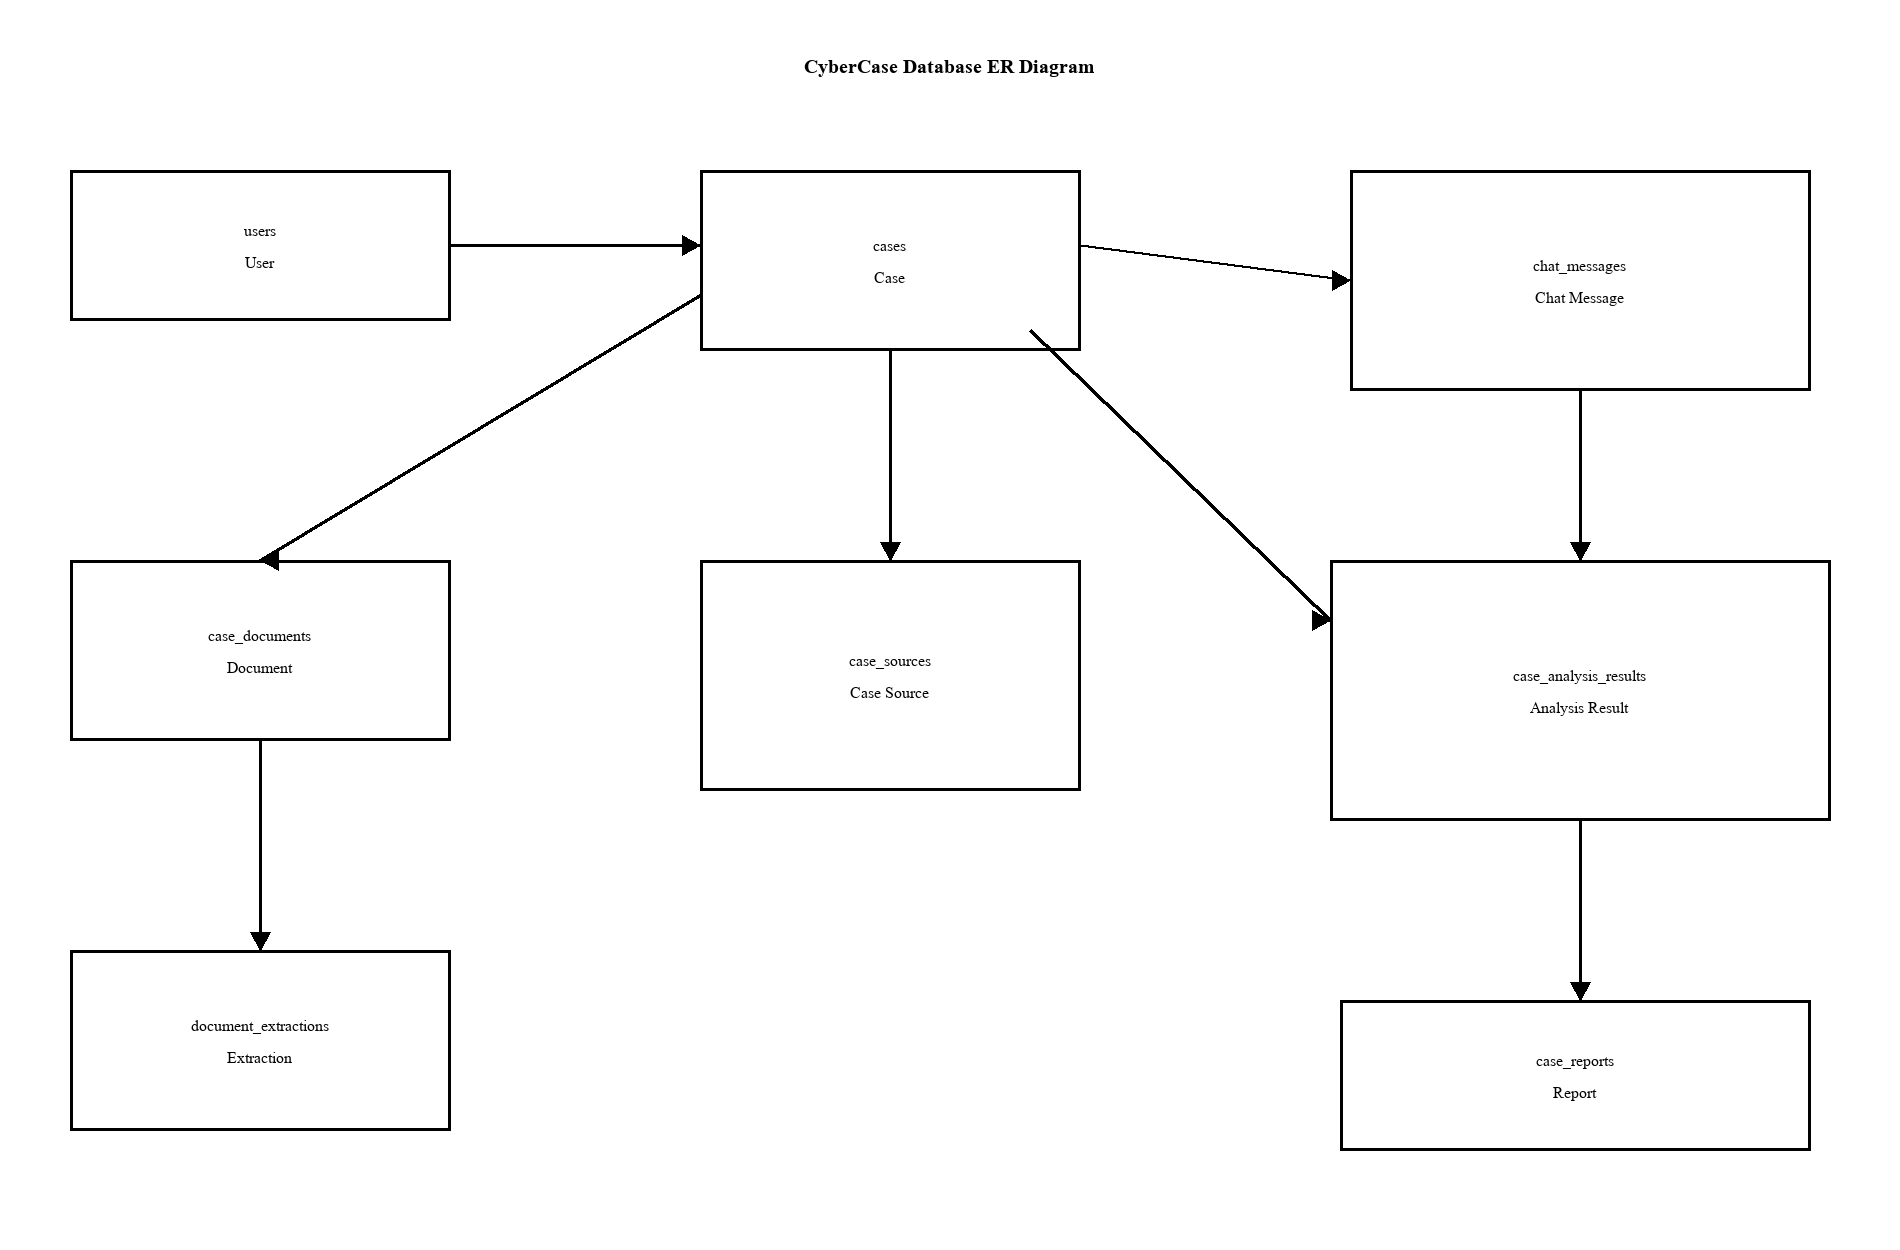
\includegraphics[width=0.96\textwidth]{figures/chapter3/figure-3-8.png}
\caption{ER Diagram of the CyberCase Database}\label{fig:3-8}
\end{figure}

\section{Data Dictionary}

The following tables describe the main data structures used by the system. The data types follow PostgreSQL conventions, and foreign keys show the relationships between tables.

\begin{longtable}{@{}>{\raggedright\arraybackslash}p{0.15\textwidth} >{\raggedright\arraybackslash}p{0.19\textwidth} >{\raggedright\arraybackslash}p{0.46\textwidth} >{\raggedright\arraybackslash}p{0.14\textwidth}@{}}
\caption{User table (users)}\label{tab:3-9}\\
\toprule
\textbf{Name} & \textbf{Type} & \textbf{Description} & \textbf{Key Type} \\
\midrule
\endfirsthead
\textbf{Name} & \textbf{Type} & \textbf{Description} & \textbf{Key Type} \\
\midrule
\endhead
id & UUID & User identifier & PK \\
email & VARCHAR(255) & User email & UNIQUE \\
name & VARCHAR(255) & Display name &  \\
password\_hash & VARCHAR(512) & Password hash; the plaintext password is not stored &  \\
oauth\_provider & VARCHAR(32) & Identity provider &  \\
oauth\_subject\_id & VARCHAR(255) & User identifier from an external provider &  \\
email\_verified\_at & TIMESTAMP & Email verification time &  \\
avatar\_url & VARCHAR(1024) & Avatar URL &  \\
created\_at & TIMESTAMP & Account creation time &  \\
updated\_at & TIMESTAMP & Latest account update time &  \\
\bottomrule
\end{longtable}

\begin{longtable}{@{}>{\raggedright\arraybackslash}p{0.15\textwidth} >{\raggedright\arraybackslash}p{0.19\textwidth} >{\raggedright\arraybackslash}p{0.46\textwidth} >{\raggedright\arraybackslash}p{0.14\textwidth}@{}}
\caption{Case table (cases)}\label{tab:3-10}\\
\toprule
\textbf{Name} & \textbf{Type} & \textbf{Description} & \textbf{Key Type} \\
\midrule
\endfirsthead
\textbf{Name} & \textbf{Type} & \textbf{Description} & \textbf{Key Type} \\
\midrule
\endhead
id & UUID & Case identifier & PK \\
user\_id & UUID & Case owner & FK -> users.id \\
title & VARCHAR(255) & Case title &  \\
source\_revision & INTEGER & Revision number of the case sources &  \\
latest\_analysis\_result\_id & UUID & Current analysis result & FK: analysis \\
created\_at & TIMESTAMP & Case creation time &  \\
updated\_at & TIMESTAMP & Latest case update time &  \\
\bottomrule
\end{longtable}

\begin{longtable}{@{}>{\raggedright\arraybackslash}p{0.15\textwidth} >{\raggedright\arraybackslash}p{0.19\textwidth} >{\raggedright\arraybackslash}p{0.46\textwidth} >{\raggedright\arraybackslash}p{0.14\textwidth}@{}}
\caption{Case-document table (case\_documents)}\label{tab:3-11}\\
\toprule
\textbf{Name} & \textbf{Type} & \textbf{Description} & \textbf{Key Type} \\
\midrule
\endfirsthead
\textbf{Name} & \textbf{Type} & \textbf{Description} & \textbf{Key Type} \\
\midrule
\endhead
id & UUID & Document identifier & PK \\
case\_id & UUID & Owning case & FK -> cases.id \\
filename & VARCHAR(255) & Received filename &  \\
mime\_type & VARCHAR(160) & File media type &  \\
size\_bytes & INTEGER & File size in bytes &  \\
content\_bytes & BYTEA & Original file content &  \\
archived\_at & TIMESTAMP & Archive time &  \\
created\_at & TIMESTAMP & Document receipt time &  \\
\bottomrule
\end{longtable}

\begin{longtable}{@{}>{\raggedright\arraybackslash}p{0.15\textwidth} >{\raggedright\arraybackslash}p{0.19\textwidth} >{\raggedright\arraybackslash}p{0.46\textwidth} >{\raggedright\arraybackslash}p{0.14\textwidth}@{}}
\caption{Document-extraction table (document\_extractions)}\label{tab:3-12}\\
\toprule
\textbf{Name} & \textbf{Type} & \textbf{Description} & \textbf{Key Type} \\
\midrule
\endfirsthead
\textbf{Name} & \textbf{Type} & \textbf{Description} & \textbf{Key Type} \\
\midrule
\endhead
id & UUID & Extraction-result identifier & PK \\
document\_id & UUID & Document that was read & FK -> case\_documents.id \\
provider & VARCHAR(120) & Provider or extraction method &  \\
config\_json & JSONB & Configuration used for extraction &  \\
extracted\_text & TEXT & Extracted text &  \\
provenance\_json & JSONB & Text provenance such as page and position &  \\
warnings\_json & JSONB & Warnings produced during extraction &  \\
created\_at & TIMESTAMP & Extraction-result creation time &  \\
\bottomrule
\end{longtable}

\begin{longtable}{@{}>{\raggedright\arraybackslash}p{0.15\textwidth} >{\raggedright\arraybackslash}p{0.19\textwidth} >{\raggedright\arraybackslash}p{0.46\textwidth} >{\raggedright\arraybackslash}p{0.14\textwidth}@{}}
\caption{Case-source table (case\_sources)}\label{tab:3-13}\\
\toprule
\textbf{Name} & \textbf{Type} & \textbf{Description} & \textbf{Key Type} \\
\midrule
\endfirsthead
\textbf{Name} & \textbf{Type} & \textbf{Description} & \textbf{Key Type} \\
\midrule
\endhead
id & UUID & Case-source identifier & PK \\
case\_id & UUID & Owning case & FK: case \\
source\_kind & VARCHAR(40) & Source type such as document, narrative, or followup\_answer &  \\
document\_id & UUID & Original document when available & FK: document \\
origin\_message\_id & UUID & Originating message when available & FK: chat \\
exact\_text & TEXT & Exact source text used as input &  \\
provenance\_json & JSONB & Provenance information for the text &  \\
source\_metadata\_json & JSONB & Additional source metadata &  \\
created\_at & TIMESTAMP & Source creation time &  \\
archived\_at & TIMESTAMP & Archive time &  \\
\bottomrule
\end{longtable}

\begin{longtable}{@{}>{\raggedright\arraybackslash}p{0.15\textwidth} >{\raggedright\arraybackslash}p{0.19\textwidth} >{\raggedright\arraybackslash}p{0.46\textwidth} >{\raggedright\arraybackslash}p{0.14\textwidth}@{}}
\caption{Chat-message table (chat\_messages)}\label{tab:3-14}\\
\toprule
\textbf{Name} & \textbf{Type} & \textbf{Description} & \textbf{Key Type} \\
\midrule
\endfirsthead
\textbf{Name} & \textbf{Type} & \textbf{Description} & \textbf{Key Type} \\
\midrule
\endhead
id & UUID & Message identifier & PK \\
case\_id & UUID & Owning case & FK -> cases.id \\
client\_request\_id & VARCHAR(255) & Client request identifier used to prevent duplicates & UNIQUE per case \\
ordinal & INTEGER & Message order within the case &  \\
role & VARCHAR(16) & User or assistant role &  \\
content & TEXT & Message content &  \\
message\_kind & VARCHAR(32) & conversation, followup\_question, or followup\_answer &  \\
gap\_key & VARCHAR(160) & Gap addressed by the question &  \\
analysis\_result\_id & UUID & Related analysis result & FK: analysis \\
in\_reply\_to\_message\_id & UUID & Message being answered & FK -> chat\_messages.id \\
metadata\_json & JSONB & Additional message data &  \\
created\_at & TIMESTAMP & Message creation time &  \\
\bottomrule
\end{longtable}

\begin{longtable}{@{}>{\raggedright\arraybackslash}p{0.15\textwidth} >{\raggedright\arraybackslash}p{0.19\textwidth} >{\raggedright\arraybackslash}p{0.46\textwidth} >{\raggedright\arraybackslash}p{0.14\textwidth}@{}}
\caption{Case-analysis-result table (case\_analysis\_results)}\label{tab:3-15}\\
\toprule
\textbf{Name} & \textbf{Type} & \textbf{Description} & \textbf{Key Type} \\
\midrule
\endfirsthead
\textbf{Name} & \textbf{Type} & \textbf{Description} & \textbf{Key Type} \\
\midrule
\endhead
id & UUID & Analysis-result identifier & PK \\
case\_id & UUID & Owning case & FK: case \\
source\_revision & INTEGER & Source revision used for analysis &  \\
schema\_version & VARCHAR(80) & Analysis contract version &  \\
status & VARCHAR(24) & assessment or validated &  \\
answer & TEXT & Analysis answer or message &  \\
summary & TEXT & Case summary &  \\
trace\_json & JSONB & Structured analysis trace &  \\
retrieval\_context\_id & VARCHAR(160) & MITRE context identifier used &  \\
retrieval\_context\_json & JSONB & Stored MITRE context for reuse &  \\
pipeline\_config & JSONB & Pipeline configuration &  \\
external\_context\_json & JSONB & External context and augmentation status &  \\
created\_at & TIMESTAMP & Analysis-result creation time &  \\
\bottomrule
\end{longtable}

\begin{longtable}{@{}>{\raggedright\arraybackslash}p{0.15\textwidth} >{\raggedright\arraybackslash}p{0.19\textwidth} >{\raggedright\arraybackslash}p{0.46\textwidth} >{\raggedright\arraybackslash}p{0.14\textwidth}@{}}
\caption{Case-report table (case\_reports)}\label{tab:3-16}\\
\toprule
\textbf{Name} & \textbf{Type} & \textbf{Description} & \textbf{Key Type} \\
\midrule
\endfirsthead
\textbf{Name} & \textbf{Type} & \textbf{Description} & \textbf{Key Type} \\
\midrule
\endhead
id & UUID & Report identifier & PK \\
case\_id & UUID & Owning case & FK: case \\
analysis\_result\_id & UUID & Analysis used to create the report & FK: analysis \\
version\_number & INTEGER & Case-level report version & UNIQUE per case \\
structured\_report & JSONB & Report in the defined structure &  \\
created\_at & TIMESTAMP & Report creation time &  \\
\bottomrule
\end{longtable}

\section{Summary of Procedures and Implementation Methods}

CyberCase starts by receiving case information and creating traceable case sources. It then performs structured analysis while deterministic rules control follow-up questions, MITRE context retrieval, and the relationship between analysis results and sources. The system can therefore present summaries and preliminary reports together with the status of uncertain information without treating external knowledge as a case fact.
